\tableofcontents
\section*{Предисловие}
При выполнении данной лабораторной работы было решено использовать 
\href{https://python-control.readthedocs.io/en/0.9.4/}{Python Control Systems Library}.
Данный инструмент является альтернативой Matlab, адаптированной для использования на 
языке Python и предоставляет широкий функционал для анализа и моделирования систем,
а также синтеза регуляторов для управления.

Полный листинг моделирования систем представлен в \href{https://github.com/diuzhevVlad/control-theory-itmo-fall-2023/blob/main/Lab9/Lab9.ipynb}{jupyter notebook} на GitHub.

\pagebreak

\section{Регулятор с заданной степенью устойчивости}
Рассмотрим систему:
\begin{equation}
    \dot{x} = Ax + Bu
\end{equation}
Матрицы $A$ и $B$ из ЛР №8:
\begin{equation*}
    A = \begin{bmatrix}
        -1 & 0 & 0 & 0 \\
        0 & 2 & 0 & 0 \\
        0 & 0 & 3 & 4 \\
        0 & 0 & -4 & 2
    \end{bmatrix},
    B = \begin{bmatrix}
        0 \\ 5 \\ 0 \\ 6
    \end{bmatrix}
\end{equation*}
Напомним, что все собственные числа, кроме $-1$ являются управляемыми. Это значит, что мы не 
сможем получить степень усточивости выше 1. Зададимся набором желаемых степеней устойчивости:
\{$0.1,0.3,0.7,1$\}.

Для синтеза регулятора с заданной степенью устойчивости $\alpha$ необходимо найти матрицы $P$ и $Y$,
удовлетворяющие неравенствам:
\begin{equation}
    P \succ 0, PA^T + AP +2\alpha P + Y^TB^T + BY \prec 0
\end{equation}
Затем, получим матрицу $K$:
\begin{equation}
    K = YP^{-1}
\end{equation}

\begin{table}[h!]
    \centering
    \begin{tabular}{| l | l | l |} 
        \hline
        $\alpha$ & $K$ & $\sigma(A+BK)$  \\  
        \hline\hline
        $0.1$ & $\begin{bmatrix} 0 & -1.63 & -2.79 & -0.22\end{bmatrix}$ & $\{-0.47+6.89i, -0.47-6.89i, -0.59 , -1\}$ \\ 
        \hline
        $0.3$ & $\begin{bmatrix} 0 & -1.95 & -3.22 & -0.07\end{bmatrix}$ & $\{-0.70+7.19i, -0.704-7.19i, -0.81 , -1\}$ \\
        \hline
        $0.7$ & $\begin{bmatrix} 0 & -2.57 & -3.99 & 0.25\end{bmatrix}$ & $\{-1.08+7.71i, -1.082-7.71i, -1.17 , -1\}$ \\
        \hline
        $1$ & $\begin{bmatrix} 0 & -3.15 & -4.66 & 0.59 \end{bmatrix}$ & $\{-1.37+8,14i, -1.378-8,14i, -1.46 , -1\}$ \\
        \hline
       \end{tabular}
    \caption{Результаты синтеза регулятора с заданными степенями устойчивости.}
    \label{table:1}
\end{table}

Выполним моделирование системы с 
входным воздействием $u = Kx$ при начальных условиях $x(0)=[1, 1, 1, 1]^T$.
\begin{figure}[]
    \centering
    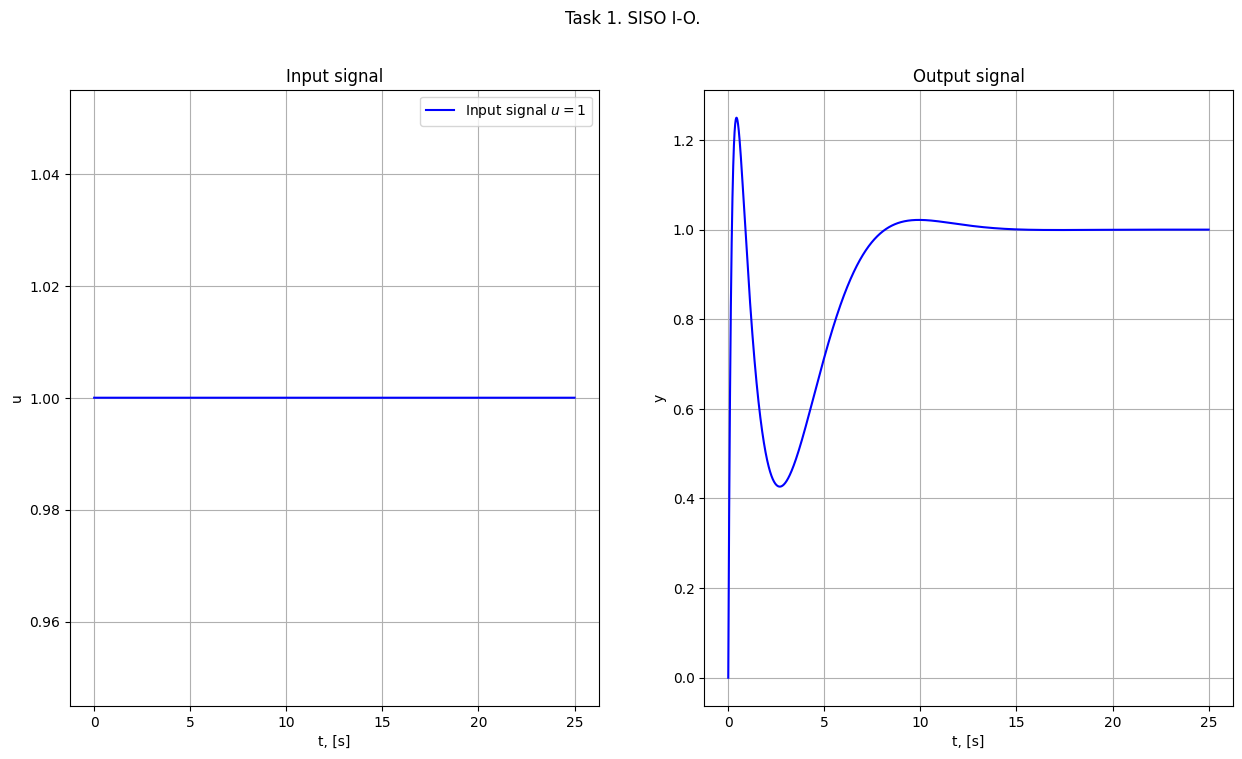
\includegraphics[width=300px]{plot_1_1.png}
    \caption{\label{fig:The-caption-1}Задание 1. Компоненты вектора состояний при различных степенях устойчивости регулятора.}
\end{figure}
\begin{figure}[]
    \centering
    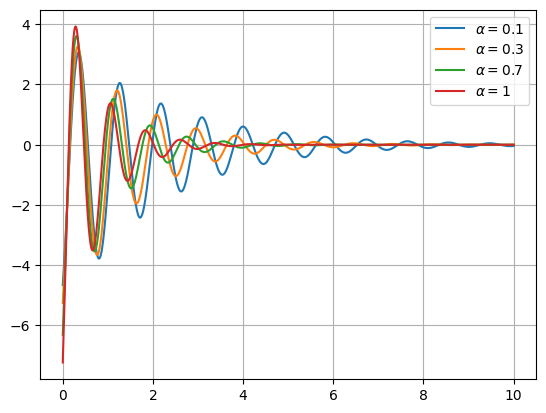
\includegraphics[width=300px]{plot_1_2.png}
    \caption{\label{fig:The-caption-1}Задание 1. Управляющий сигнал при различных степенях устойчивости регулятора.}
\end{figure}
\pagebreak

\section{Регулятор с ограниченным управлением}
Зададимся набором ограничений для управляющего воздействия ($\mu$) при
начальных условиях $x(0)$: \{$9,8,7,6$\}. Для
синтеза регулятора с ограничением на управляющее воздействие к неравенствам (2) добавляются
следующие:
\begin{equation}
    \begin{bmatrix}
        P & x(0) \\
        x(0)^T & 1
    \end{bmatrix} \succ 0,
    \begin{bmatrix}
        P & Y^T \\
        Y & \mu^2
    \end{bmatrix} \succ 0
\end{equation}
Зафиксируем $\alpha=0.7$.
\begin{table}[h!]
    \centering
    \begin{tabular}{| l | l | l |} 
        \hline
        $\mu$ & $K$ & $\sigma(A+BK)$  \\  
        \hline\hline
        $9$ & $\begin{bmatrix} 0 & -1.52 & -2.62 & -0.58\end{bmatrix}$ & $\{-1.04+5.79i, -1.04-5.79i, -1.017  , -1\}$ \\ 
        \hline
        $8$ & $\begin{bmatrix} 0 & -1.34 & -2.37 & -0.71\end{bmatrix}$ & $\{-0.99+5.44i, -0.99-5.44i, -0.97  , -1\}$ \\
        \hline
        $7$ & $\begin{bmatrix} 0 & -1.48 & -2.55 & -0.54\end{bmatrix}$ & $\{-0.89+5.92i, -0.89-5.92i, -0.91 , -1\}$ \\
        \hline
        $6$ & $\begin{bmatrix} 0 & -1.34 & -2.35 & -0.59 \end{bmatrix}$ & $\{-0.76+5.79i, -0.76-5.79i, -0.77 , -1\}$ \\
        \hline
       \end{tabular}
    \caption{Результаты синтеза регулятора с заданными ограничениями управляющего воздействия.}
    \label{table:2}
\end{table}
\begin{figure}[h]
    \centering
    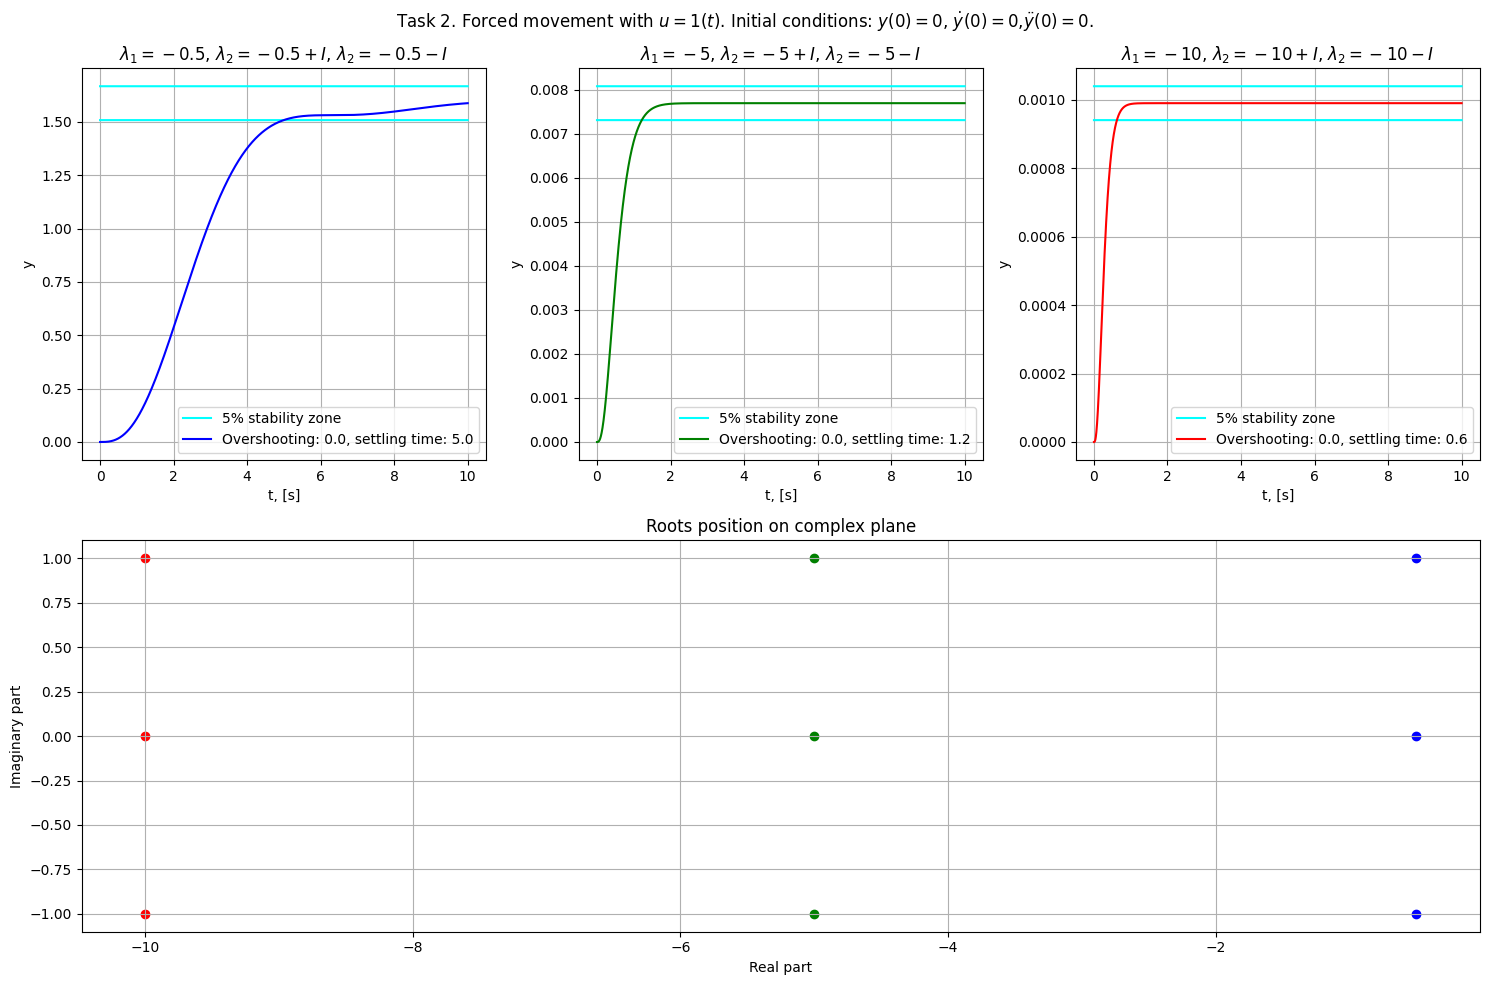
\includegraphics[width=300px]{plot_2_3.png}
    \caption{\label{fig:The-caption-1}Задание 2. Компоненты вектора состояний при различных ограничениях.}
\end{figure}
\begin{figure}[h]
    \centering
    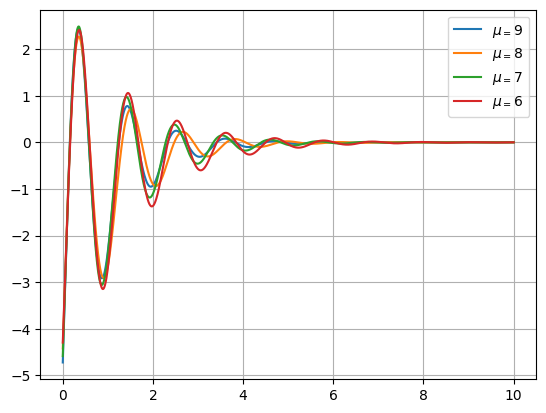
\includegraphics[width=300px]{plot_2_4.png}
    \caption{\label{fig:The-caption-1}Задание 2. Управляющий сигнал при различных ограничениях.}
\end{figure}
\pagebreak

Добавим к условиям (2) и (4) необходимость минимизации $\mu$.
\begin{table}[h!]
    \centering
    \begin{tabular}{| l | l | l | l |} 
        \hline
        $\alpha$ & $\mu_{min}$ & $K$ & $\sigma(A+BK)$  \\  
        \hline\hline
        $0.1$ & $4.24$ & $\begin{bmatrix} 0 & -0.86 & -1.64 & -0.66\end{bmatrix}$ & $\{-0.099+5.525i, -0.099-5.525i, -0.104  , -1\}$ \\ 
        \hline
        $0.3$ & $4.79$ & $\begin{bmatrix} 0 & -1.03 & -1.91 & -0.62\end{bmatrix}$ & $\{-0.299+5.725i, -0.299-5.725i, -0.301  , -1\}$ \\
        \hline
        $0.7$ & $6.02$ & $\begin{bmatrix} 0 & -1.43 & -2.49 & -0.49\end{bmatrix}$ & $\{-0.701+6.137i, -0.701-6.137i, -0.705, -0.91 , -1\}$ \\
        \hline
        $1$ & $7.05$ & $\begin{bmatrix} 0 & -1.78 & -2.98 & -0.34 \end{bmatrix}$ & $\{-1+6.458i, -1-6.458i, -1 , -1\}$ \\
        \hline
       \end{tabular}
    \caption{Результаты синтеза регулятора с минимизации ограничений управляющего воздействия.}
    \label{table:3}
\end{table}
\begin{figure}[]
    \centering
    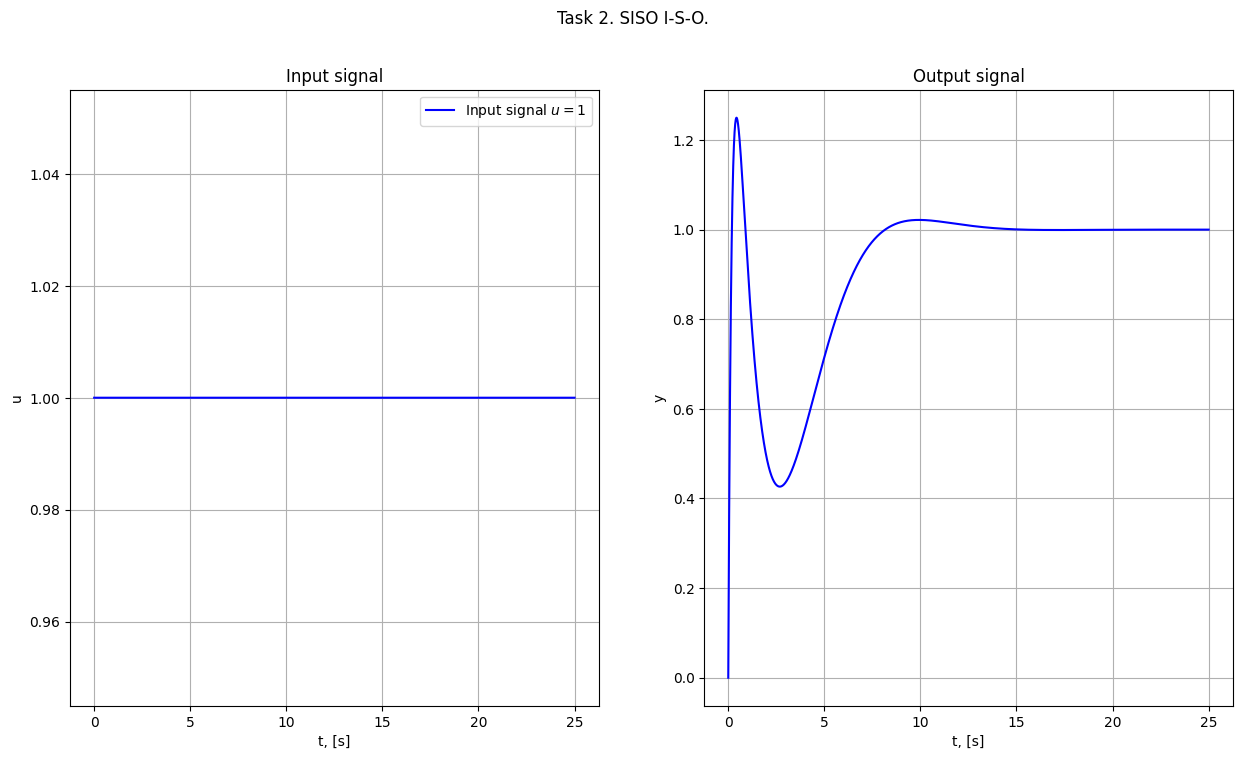
\includegraphics[width=300px]{plot_2_1.png}
    \caption{\label{fig:The-caption-1}Задание 2. Компоненты вектора состояний при минимальных ограничениях.}
\end{figure}
\begin{figure}[]
    \centering
    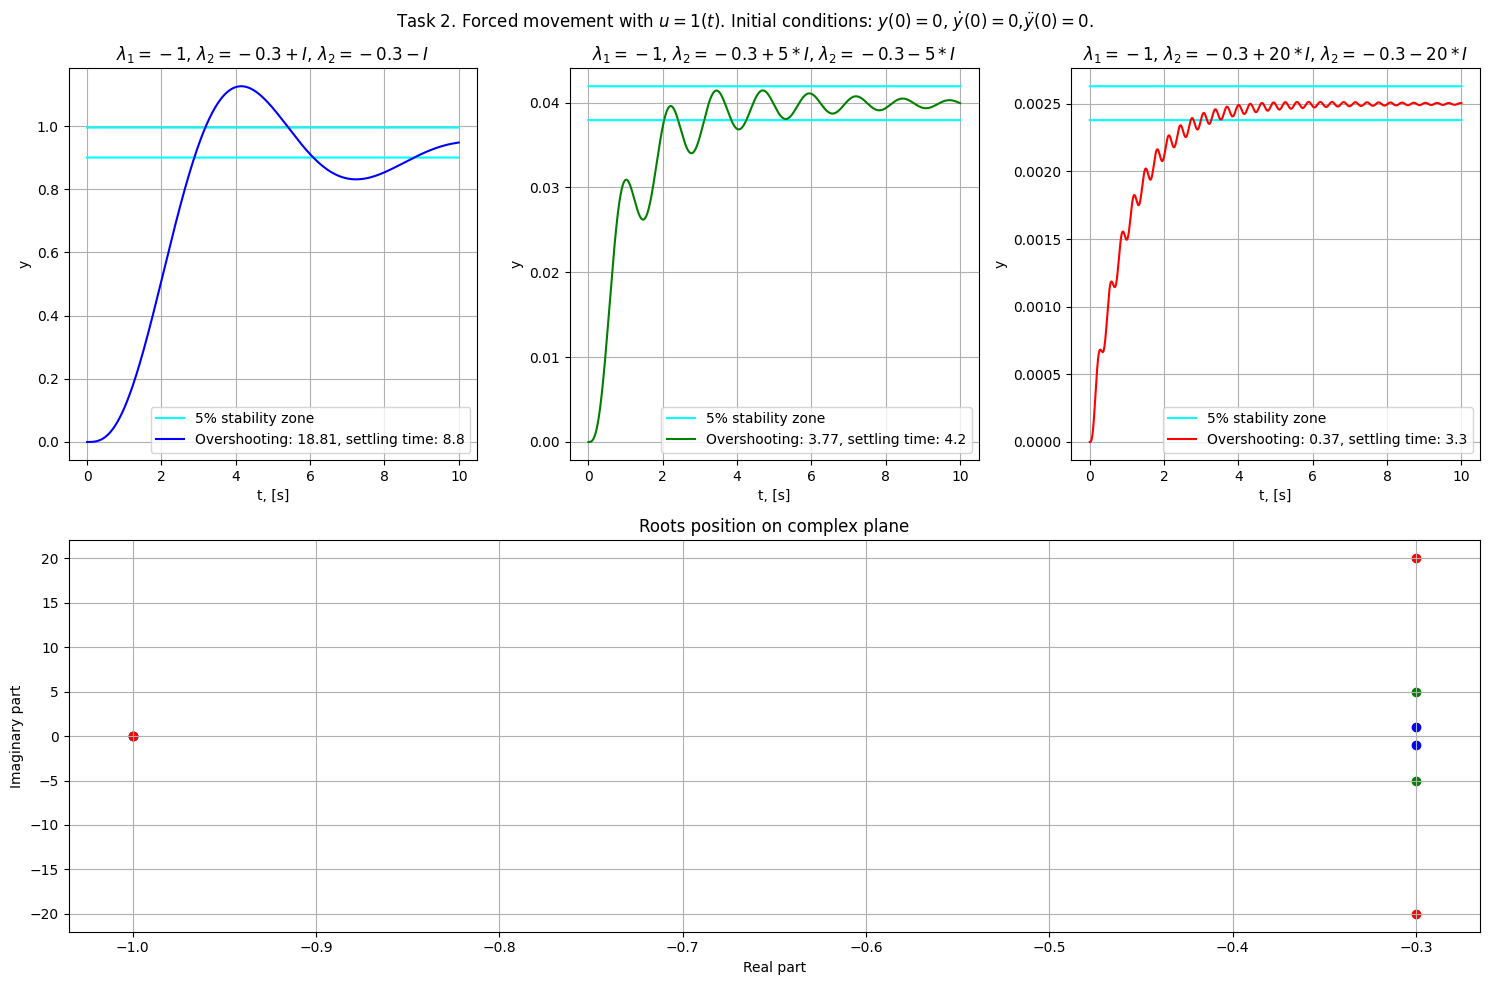
\includegraphics[width=300px]{plot_2_2.png}
    \caption{\label{fig:The-caption-1}Задание 2. Управляющий сигнал при минимальных ограничениях.}
\end{figure}

Проведем моделирование систем с полученными коэффициентами регулятора.
\pagebreak

\section{Наблюдатель с заданной степенью устойчивости}
Рассмотрим систему:
\begin{equation}
    \dot{x} = Ax, y = Cx
\end{equation}
Матрицы $A$ и $C$ (как показано в ЛР №8, пара -- полностью наблюдаема):
\begin{equation*}
    A = \begin{bmatrix}
        0 & 3 & 0 & 0 \\
        -3 & 0 & 0 & 0 \\
        0 & 0 & 0 & 1 \\
        0 & 0 & -1 & 0
    \end{bmatrix},
    C = \begin{bmatrix}
        2 & 0 & 0 & 3
    \end{bmatrix}
\end{equation*}

Зададимся набором желаемых степеней устойчивости:
\{$1,3,6,9$\}.

Для синтеза наблюдателя с заданной степенью устойчивости $\alpha$ необходимо найти матрицы $Q$ и $Y$,
удовлетворяющие неравенствам:
\begin{equation}
    Q \succ 0, A^TQ + QA +2\alpha Q + C^TY^T + YC \prec 0
\end{equation}
Затем, получим матрицу $L$:
\begin{equation}
    L = Q^{-1}Y
\end{equation}

\begin{table}[h!] 
    \centering
    \begin{tabular}{| l | l | l |} 
        \hline
        $\alpha$ & $L$ & $\sigma(A+LC)$  \\  
        \hline\hline
        $1$ & $\begin{bmatrix} 1.31 & -2.69 & 2.17 & -2.72\end{bmatrix}^T$ & $\{-1.33+4.39i, -1.33-4.39i, -1.43+1.39i, -1.43-1.39i\}$ \\ 
        \hline
        $3$ & $\begin{bmatrix} 43.51 & 1.9 & 58.26 & -34.21\end{bmatrix}^T$ & $\{-4.17+8.89i, -4.17-8.89i, -3.63+1.76i, -3.63-1.76i\}$ \\
        \hline
        $6$ & $\begin{bmatrix} 430.24 & 412.21 & 1064.31 & -297.3\end{bmatrix}^T$ & $\{-8.48+18.71i, -8.48-18.71i, -7.24+3.13i, -7.24-3.13i\}$ \\
        \hline
        $9$ & $\begin{bmatrix} 1404.68 & 2235.75 & 4998.16 & -952.19\end{bmatrix}^T$ & $\{-12.8+27.2i, -12.8-27.2i, -10.8+4.3i, -10.8-4.3i\}$ \\
        \hline
       \end{tabular}
    \caption{Результаты синтеза наблюдателя с заданными степенями устойчивости.}
    \label{table:1}
\end{table}


Проведем моделирование систем с полученными коэффициентами наблюдателя.

\begin{figure}[]
    \centering
    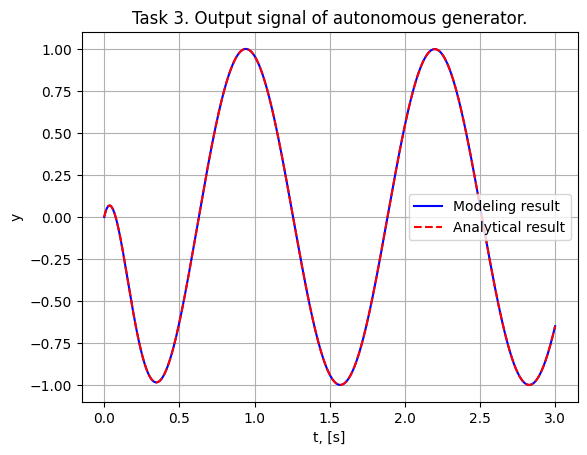
\includegraphics[width=300px]{plot_3_1.png}
    \caption{\label{fig:The-caption-1}Задание 3. Компоненты вектора состояний системы и наблюдателей разных степеней устойчивости.}
\end{figure}
\begin{figure}[]
    \centering
    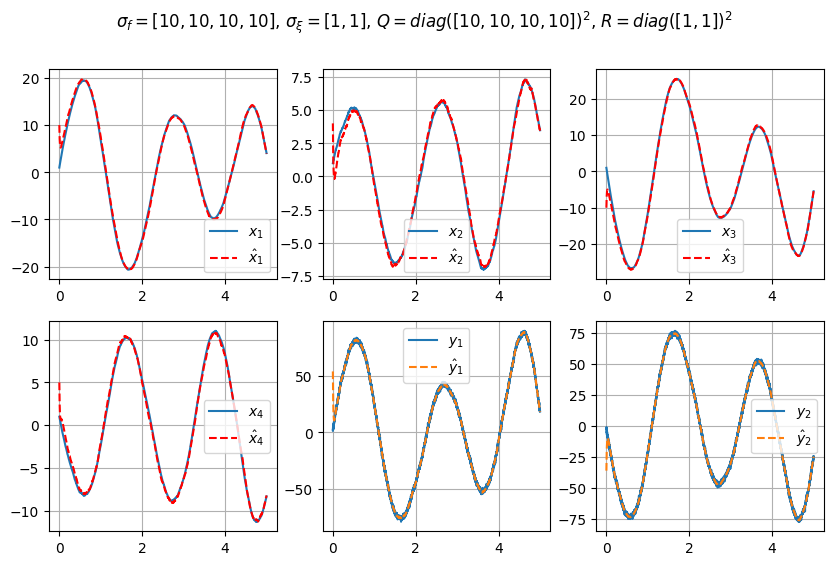
\includegraphics[width=300px]{plot_3_2.png}
    \caption{\label{fig:The-caption-1}Задание 3. Ошибки наблюдателей разных степеней устойчивости.}
\end{figure}

\pagebreak

\section{Совместный синтез регулятора и наблюдателя}
Рассмотрим систему:
\begin{equation}
    \begin{cases}
        \dot x = Ax + Bu \\
        y = Cx
    \end{cases}
\end{equation}
Матрицы $A$, $B$ и $C$:
\begin{equation*}
    A = \begin{bmatrix}
        3 & -11 & -7 & 5 \\
        -11 & 3 & -5 & 7 \\
        -7 & -5 & 3 & 11 \\
        5 & 7 & 11 & 3
    \end{bmatrix},
    B = \begin{bmatrix}
        2 \\ 4 \\ 2 \\ 4
    \end{bmatrix},
    C = \begin{bmatrix}
        3 & -2 & 2 & 2 \\
        2 & 4 & -2 & 4
    \end{bmatrix}
\end{equation*}
На основании анализа из ЛР №8 система является полностью управляемой, однако частично наблюдаемой 
(собственное число -20 не является наблюдаемым). Заметим, что нам не удастся синтезировать наблюдатель степени устойчивости выше 20.

Зафиксируем степень устойчивости регулятора $\alpha_{cont}=2$ и рассмотрим 3 характерных случая:
\begin{enumerate}
    \item степень устойчивости наблюдателя меньше степени устойчивости регулятора ($\alpha_{obs}=0.5$)
    \item степень устойчивости наблюдателя равна степени устойчивости регулятора ($\alpha_{obs}=2$)
    \item  степень устойчивости наблюдателя больше степени устойчивости регулятора ($\alpha_{obs}=4$)
\end{enumerate}

Выполним моделирование систем.
\begin{figure}[h]
    \centering
    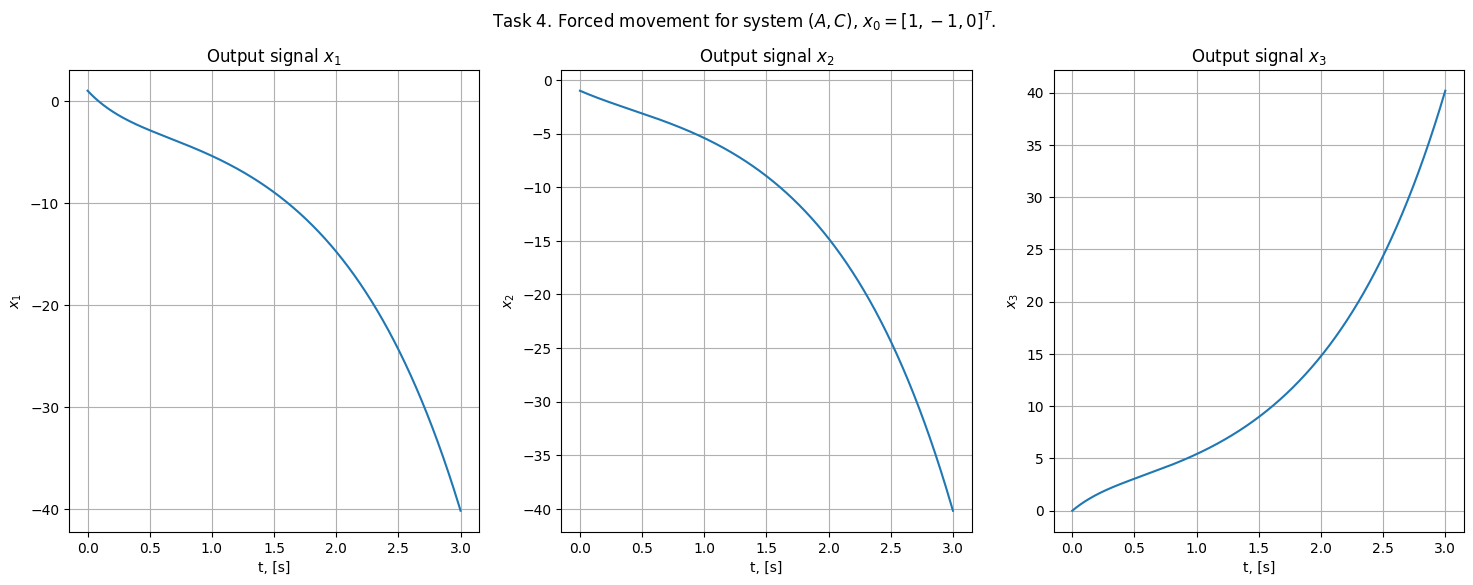
\includegraphics[width=300px]{plot_4_1.png}
    \caption{\label{fig:The-caption-1}Задание 4. Компоненты вектора состояний системы и наблюдателя ($\alpha_{cont} > \alpha_{obs}$).}
\end{figure}
\begin{figure}[]
    \centering
    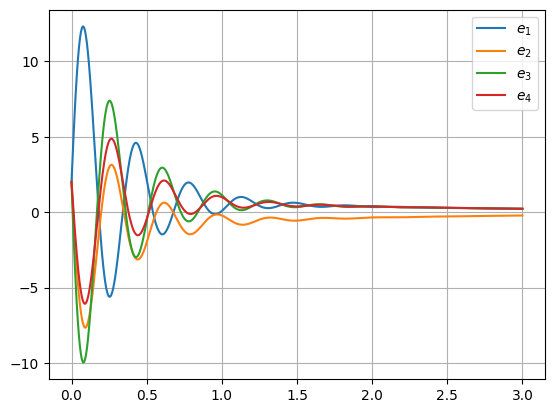
\includegraphics[width=300px]{plot_4_2.png}
    \caption{\label{fig:The-caption-1}Задание 4. Ошибки наблюдателя ($\alpha_{cont} > \alpha_{obs}$).}
\end{figure}
\begin{figure}[]
    \centering
    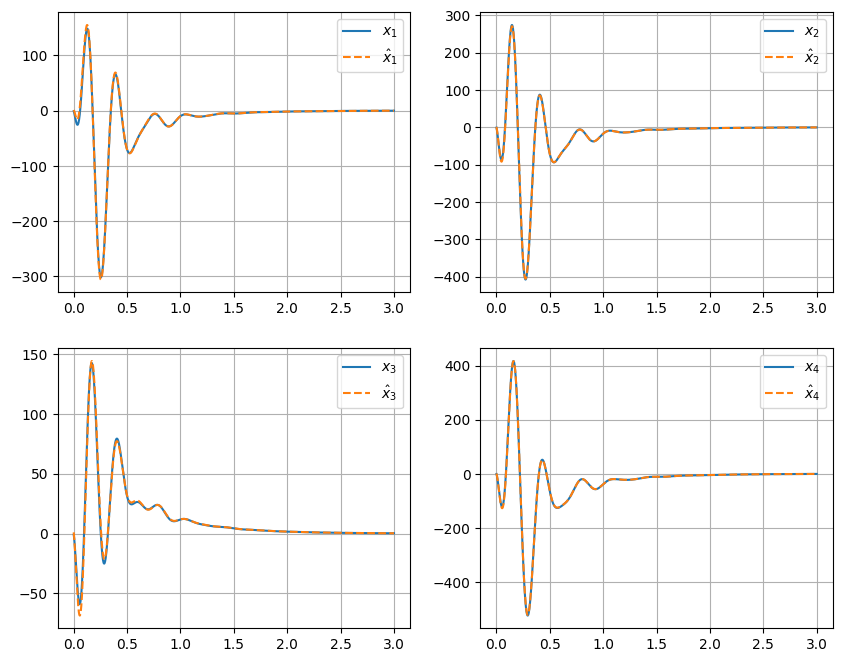
\includegraphics[width=300px]{plot_4_3.png}
    \caption{\label{fig:The-caption-1}Задание 4. Компоненты вектора состояний системы и наблюдателя ($\alpha_{cont} = \alpha_{obs}$).}
\end{figure}
\begin{figure}[]
    \centering
    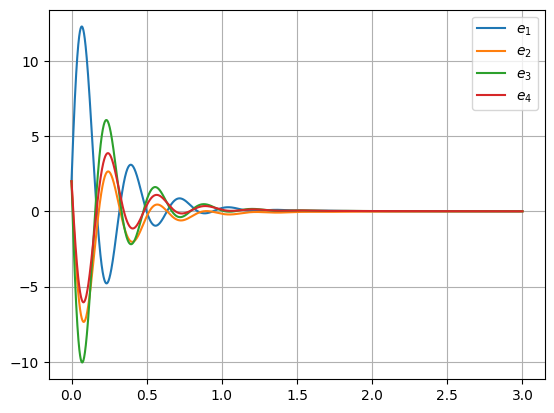
\includegraphics[width=300px]{plot_4_4.png}
    \caption{\label{fig:The-caption-1}Задание 4. Ошибки наблюдателя ($\alpha_{cont} = \alpha_{obs}$).}
\end{figure}
\begin{figure}[]
    \centering
    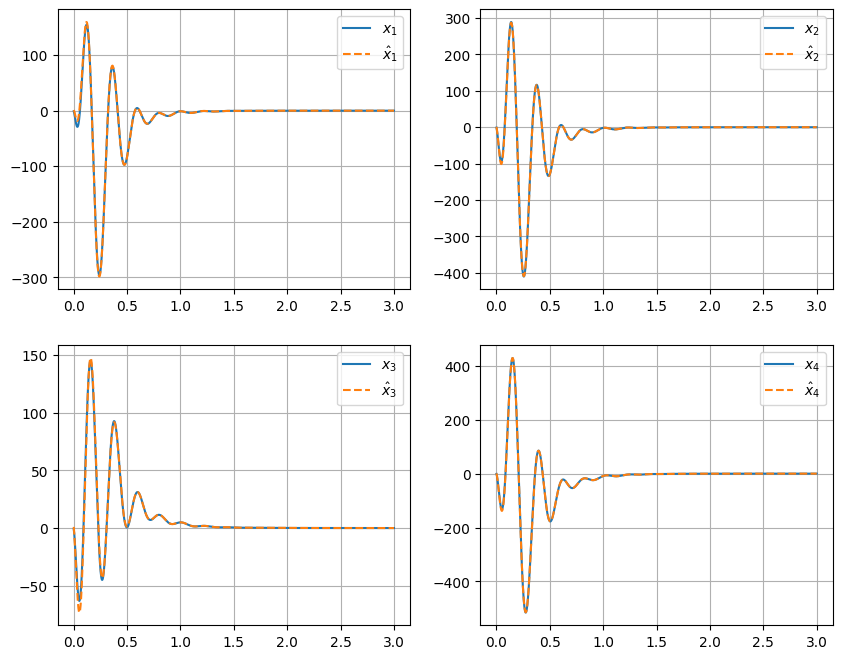
\includegraphics[width=300px]{plot_4_5.png}
    \caption{\label{fig:The-caption-1}Задание 4. Компоненты вектора состояний системы и наблюдателя ($\alpha_{cont} < \alpha_{obs}$).}
\end{figure}
\begin{figure}[]
    \centering
    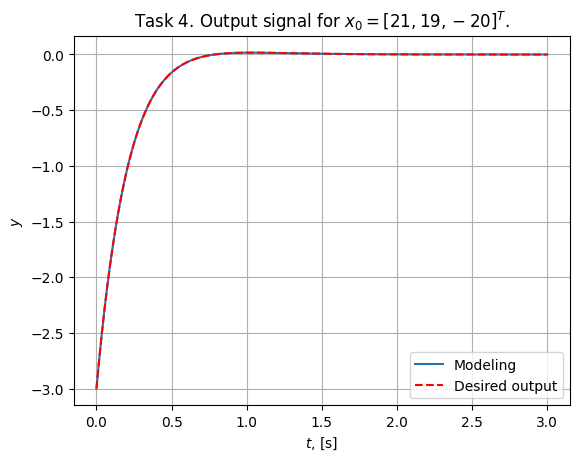
\includegraphics[width=300px]{plot_4_6.png}
    \caption{\label{fig:The-caption-1}Задание 4. Ошибки наблюдателя ($\alpha_{cont} < \alpha_{obs}$).}
\end{figure}
\pagebreak

\section{Выводы}
В ходе выполнения данной лабораторной работы получили навыки синтеза регуляторов и наблюдателей с заданной степенью устойчивости
с помощью аппарата линейных матричных неравенств.
\begin{enumerate}
    \item Ограничение на степень устойчивости регуляторов и наблюдателей обусловлено наличем неуправляемых/ненаблюдаемых
собственных чисел матрицы системы.
    \item При наложении условия ограниченности входного воздействия при синтезе регулятора можем заметить увеличение
действительной части собственных чисел матрицы $A + BK$. При минимизации входного воздействия, данные значения становятся близки к заданной степени устойчивости.
    \item Высокие степени устойчивости набюдателей гарантируют быструю сходимость, однако в начале переходного процесса
ошибка наблюдателя может быть существенно больше допустимой в реальных системах.
    \item Различные конфигурации степеней устойчивости регуляторов и наблюдателей влияют на сходимость системы ошибки наблюдателя. В случае
когда степень устойчивости наблюдателя меньше степени устойчивости регулятора можем наблюдать существенно более длительный переходный процесс системы и ошибки.
\end{enumerate}